\subsection{Overview}
Given a finite sample, the \emph{sample covariance matrix} $\hat\Sigma_0$ is the usual estimator of the \emph{true covariance matrix} $\Sigma$ of the underlying random process.  $\hat\Sigma_0$ is unbiased but, with finite sample sizes, not as close to $\Sigma$ as possible.  More \emph{efficient} estimators can be constructed by \emph{regularization}, which is the deliberate biasing of the usual estmate toward a different, low-dimensional parametric \emph{target estimate} $\hat T$. 
Target estimates are biased approximations because they cannot represent an arbitrary $\Sigma$, but they also have lower random variability.
Regularization reduces the overall error by striking a favorable balance between the variance  (\emph{estimation error}) and the bias \emph{(approximation error)} of the estimate.  
  
A regularized estimate requires the following three choices: 
\begin{enumerate}[  1. ]
\item define a set of low-dimensional target estimates
\item given the data, select the optimal target estimate from the set 
\item given the data, select the optimal amount of biasing toward the target estimate
\end{enumerate}
The first choice, the selection of the general form of target estimates, must be made \emph{a priori}.  Curiously, \emph{some} improvement can be produced with an arbitrary target estimate as long as its variance is lower than that of the unbiased estimator.  The perplexing fact that estimates can be improved by biasing toward an arbitrary less variable target is known as \emph{Stein's paradox} \citep{Efron:1977}.  


\subsection{Probabilistic framework}
\TODO{This section is not strictly necessary. It helps relate probabilistic models to our approach, which does not rely on an explicity probabilistic model.}
Let $x_i \in \mathcal X, i=1\ldots,x_n$ denote a sample of consequtive observations of population activity of $p$ neurons in time bins $i$.  
The activity of each neuron is the real-valued firing rate \TODO{Need to define rate more precisely}, thus  $\mathcal X = \mathbb R^{p\times 1}$.  
We assume that observations are drawn from some true cumulative probability distribution $F: \mathcal X \mapsto R$. Then let $\hat F_n$ denote the empirical distribution function obtained from the observed sample, which itself is a random variable.
\begin{equation}
\hat F_n(x) = \frac 1 n \sum\limits_{i=1}^n \mathbf{1}(x \ge x_i)
\end{equation}
where $\mathbf 1(x \ge x_i)$ is the indicator function which equals 1 when all elements of $x$ are greater than the corresponding elements of $x_i$ and 0 otherwise. \TODO{KJ: Are you using cumulative distributions to avoid binning? DY: Yes. Many theorems such as Glivenko-Catelli Theorem and Skorohod's Representation are proven using  cumulative representation. The empirical distribution is nearly always represented in its cumulative form. Expressing convergence is requires binning or using cumulative; the latter is simpler.}

The observations need not be independently and identically sampled from $F$. The only assumption is that the data generating process is ergodic, \emph{i.e.}\;that $\max\limits_x \left[\hat F_n(x) - F(x)\right] \to 0$ as the sample size $n$ increases. Then each $x_i$ can be thought to be drawn from $F$ when not conditioned on nearby observations.

The true covariance matrix $\Sigma \in \Theta$ is defined as a function of the true probability distribution
\begin{equation}
\Sigma = \int\limits_{z\in\mathcal X} (z - \bar x)(z - \bar x)^\T \dif F(z)
\quad\mbox{where}\;
\bar x = \int\limits_{z\in\mathcal X} z \dif F(z)
\end{equation}
The \emph{plug-in estimator} $\hat\Sigma$ is obtained by plugging the empirical distribution $F_n$ in place of the true distribution $F$
\begin{equation}
\begin{split}
\hat\Sigma = \int\limits_{z\in\mathcal X} (z - \bar x)(z - \bar x)^\T \dif \hat F_n(z) 
\equiv \frac  1 n\sum\limits_{i=1}^n (x_i-\bar x)(x_i - \bar x)
\\
\mbox{where}\;\bar x = 
\int\limits_{z\in \mathcal X}z \dif \hat F_n(z) \equiv \frac 1 n\sum\limits_{i=1}^n x_i
\end{split}
\end{equation}
The plug-in estimator is known to be biased toward zero because the estimate of the mean $\bar x$ absorbs a fraction of the variances. 

The usual unbiased estimate, the sample covariance matrix, rescales the plug-in estimator to compensate for the bias
\begin{equation}
\hat\Sigma_0 = \frac n {n - d} \hat\Sigma \equiv \frac 1 {n-d} \sum\limits_{i=1}^n (x_i - \bar x) (x_i - \bar x)^\T
\end{equation}
When observations are independent, then $d=1$.  But when nearby samples are correlated, the estimate of the mean absorbs more of the variance, becomes \emph{overdispersed}. As a result the covariances become underestimated. Then we can use $d=cn$ where $c>1$ is called the \emph{overdispersion coefficient}, which may be estimated from the data.

\subsection{Measures of error}
Let $\hat\Sigma_\gamma$ be a family of approximate (biased) covariance estimates indexed by $\gamma$. To evaluate each estimate, let's define the \emph{loss function} $\mathcal L : \Theta \times \Theta \mapsto \mathbb R$ such that $\mathcal L(\hat S,S)$ is minimized when $\hat S = S$.  Then \emph{excess loss} $\ell(\hat S, S) = \mathcal L(\hat S, S) - \mathcal L(S,S)$ assumes zero at the minimum. \TODO{This is too abstract -- need to motivate with some examples maybe}

The overall error or \emph{estimator risk} 
\begin{equation}
r_\gamma = \mathbb E\left[ \ell\left(\hat\Sigma_\gamma,\Sigma\right) \right]
\end{equation}
can be decomposed into \emph{approximation error} or \emph{bias}   
\begin{equation}
b_\gamma^2 = \ell \left( \mathbb E\left[\hat \Sigma_\gamma\right],\Sigma\right)
\end{equation}
and \emph{estimation error} or \emph{variance}
\begin{equation}
\varepsilon_\gamma^2 = \mathbb E \left[ \ell\left(\hat \Sigma_\gamma, 
\mathbb E\left[\hat \Sigma_\gamma\right]\right) \right]
\end{equation}

When the loss function is the error sum of squares, which, for matrices, is called the Frobenius norm, 
\begin{equation}
\mathcal L_e(\hat S,S) = \|\hat S-S\|_F^2 = \Tr\left((\hat S-S)(\hat S-S)^\T\right)
\end{equation}
the variance-bias decomposition is the simple sum
\begin{equation}
r_\gamma =  b_\gamma^2 + \varepsilon_\gamma^2
\end{equation}

With other loss functions, the risk is also an increasing function of the two components, although is not generally the sum.

Regularization is the game of minimizing risk $r_\gamma$ by reducing estimation error $\varepsilon_\gamma$ at the cost of increased bias $b_\gamma$, the \emph{bias-variance tradeoff}.  \TODO{This point can be untuitive.  For example, \cite{Varoquaux:2012} misrepresents the effect of regularization by stating that regularization removes the upward bias of correlations in the sample covariance matrix. In reality, regularization should start with an unbiased estimator and bias it toward a low-variance target so that the estimation risk is reduced. Another important point is ``Stein's paradox'': regularization does not improve the estimate of each covariance. In fact, it makes it worse. Regularization only improves the risk when measured on the entire matrix. Regularization should not be used to improve the estimate of average correlations or the distribution of correlations.}
We follow the convention that $\hat\Sigma_{\gamma=0}$ is the unbiased estimator $\hat\Sigma_0$, \emph{i.e.}\;$b_{\gamma=0}^2 = 0$. 
We define a sequence of approximations $\hat\Sigma_\gamma$ that become less variable as as $\gamma$ increases, which is usually accompanies by increased bias. Then $\hat\Sigma_\gamma$ defines the \emph{regularization path}, for which \emph{regularization intensity} $\gamma$ specifies the location along the path, which may be real-valued or discrete, or even a vector to steer the bias toward multiple targets.  

An unbiased estimate does not guarantee lack of bias in nonlinear functions of that estimate: $\mathbb E\left[\hat\Sigma_0\right]=\Sigma \centernot\implies  E\left[\varphi(\hat\Sigma_0)\right]=\varphi(\Sigma)$, where $\varphi$ is a nonlinear function. For example, if $u_{\max}(S)$ is the largest eigevalue of square matrix $S$, then $\mathbb E\left[u_{\max}(\hat\Sigma_0)\right] > u_{\max}(\Sigma)$. Some regularization schemes have been designed to correct for the eigenspectrum bias  at the cost of adding bias to covariance coefficients \citep{Ledoit:2004}.

\paragraph{Evaluation of estimators:}
Another popular loss  function for covariance estimation arises from the theory of normal distributions.  Under the assumption of normality  with zero mean, the log likelihood of the covariance matrix $\Sigma$ given the independent sample $z_1,\ldots,z_m$, with $S = \tfrac 1 m \sum\limits_{i=1}^m z_i z_i^\T$,  
\begin{equation}
L\left(\Sigma \mid S\right) = -\tfrac m 2 \ln(2\pi) - \tfrac m 2 \ln \det \Sigma - \tfrac m 2 \Tr(\Sigma^{-1} S)
\end{equation}
Then the Gaussian loss function $\mathcal L_g$ is constructed by rescaling the normal log likelihood and dropping the constant term
\begin{equation}
\begin{split}
\mathcal L_g(\hat S,S) = &-\frac 2 m L\left(S \mid \hat S \right) - \ln(2\pi) 
\\ 
\equiv & \ln \det \hat S + \Tr(\hat S^{-1} S) 
\end{split}
\end{equation}
The corresponding excess loss 
\begin{equation}
\ell_g(\hat S,S) = \mathcal L_g(\hat S,S) - \mathcal L_g(S,S) 
= -\ln \det \left(\hat S^{-1} S\right) + \Tr\left(\hat S^{-1}S\right) - p
\end{equation}
is known as \emph{entropy loss} \citep{James:1961}.

Despite the fact that entropy loss is derived from normal theory, the choice of a loss function is not equivalent to assuming a specific form of $F$. The loss function measures the discrepancy between distribution parameters rather than the distance between distributions. \TODO{explain Bregman divergence?} 

In practice, the true covariance matrix $\Sigma$ is not available and the estimator risk must be estimated from data. This requires a separate \emph{validation} empirical distribution $\hat F_m^\prime$ of $m$ observations sampled from $F$ independently of the \emph{training} distribution $\hat F_n$. The we can produce an independent unbiased covariance estimate $\hat \Sigma_0(\hat F_m^\prime)$.

Then the \emph{empirical risk} is 
\begin{equation}
\hat r_\gamma = \mathcal L\left(\hat\Sigma_\gamma,\hat\Sigma_0(\hat F_m^\prime)\right) 
\end{equation}

 The two loss functions $\mathcal L_e(\hat S,S)$ and $\mathcal L_g(\hat S,S)$ are particularly suitable for empirical risk estimation thanks to their linearity with respect to $S$ in the sense that 
\begin{equation}
\mathcal L\left(\hat S,\alpha S_1 + (1-\alpha)S_2\right) 
\equiv 
\alpha\mathcal L(\hat S,S_1) + (1-\alpha)\mathcal L(\hat S,S_2)
\end{equation}
which allows bringing the expectation inside 
\begin{equation}
\mathbb E\left[ \mathcal L\left(\hat\Sigma_r, \hat\Sigma_0(\hat F_m^\prime)\right) \right] 
=
\mathbb E\left[ \mathcal L\left(\hat\Sigma_\gamma, \mathbb E\left[\Sigma_0(\hat F_m^\prime)\right]\right) \right] 
=
\mathbb E\left[ \mathcal L\left(\hat\Sigma_\gamma, \Sigma\right) \right] 
\end{equation}
Then the expectation of the empirical risk is 
\begin{equation}
\mathbb E\left[\hat r_\gamma\right] 
= \mathbb E\left[\mathcal L(\hat\Sigma_\gamma,\Sigma)\right]
= r_\gamma + \mathcal L(\Sigma,\Sigma)
\end{equation}
This means, that our goal of minimizing the true loss $r_\gamma$ can be replaced with minimizing  the empirical loss $\hat r_\gamma$.

In practice, recording a separate independent validation sample may not be sensible.  Instead, the recorded data a split into a training sample and validation sample. In $K$-fold \emph{cross-validation} the data are split into $K$ roughly equal-sized subsets. Each subset then successively serves to construct the validation distribution $\hat F_m^\prime$  while the rest of the data is used to construct the training distribution $\hat F_n$.  This procedure produces $K$ estimates of the empirical risk, which are then averaged together to produce a better, averaged, estimate of the true risk.

Different regularization schemes can then be compared by comparing cross-validated empirical losses.

 
\subsection{Regularization of covariance estimates}
The task of designing a regularized estimators consists of defining a sequence of approximations $\hat\Sigma_\gamma$, called \emph{regularization path} and the optimal location on that path, \emph{regularization intensity} $\hat\gamma$ as  functions of the empirical distribution. 

There are two basic approaches to design a family of approximations of a parameter that reduce the estimation error: \emph{dimensionality reduction} and \emph{shrinkage}.  

Dimensionality reduction projects the estimate onto a low-dimensional manifold (subspace) within the $p(p+1)/2$-dimensional space of covariance matrices $\Theta$.  The variance in the projection is likely to be lower (if the manifold is smooth).  For example, factor analysis with $\nu$ factors projects (w.r.t.\;$\mathcal L_g$) $\hat\Sigma_0$ onto the low-dimensional manifold of covariance matrices representable by factor models. Thus factor analysis can be used as a regularized covariance estimator \citep{Fan:2008} with $\gamma$ controlling the number of factors (or, alternatively, the nuclear norm).  Another dimensionality reduction technique is \emph{covariance selection} \citep{Dempster:1972}, wherein a fraction of inverse covariance coefficients are constrained to zero and the closest (w.r.t.\;$\mathcal L_g$) solution to $\hat\Sigma_0$ is found. 

Covariance shrinkage \citep{Schafer:2005,Ledoit:2004} uses a fixed, low-dimensional \emph{target estimate} $T$ and constructs the estimator as the linear mixture, with $\gamma \in [0,1]$,
\begin{equation}
\hat\Sigma_\gamma = \hat\Sigma_0  + \gamma (T-\hat\Sigma_0) 
\end{equation}
 The target can be a diagonal matrix with sample variances, an identity matrix scaled to the mean variance, a single factor model, or any other low-dimensional estimate.

An effective hybrid of dimensionality reduction and shrinkage can be obtained by using $L_1$-regularization techniques.  For example, graphical lasso \citep{Meinshausen:2006,Friedman:2008}, shrinks the inverse of the covariance toward zero as 
\begin{equation}
\hat\Sigma_\gamma = \arg\min\limits_S \mathcal L_g(S,\hat \Sigma_0) + \gamma \| S^{-1} \|_1
\end{equation}
This approach results in forcing many of the coefficients in the inverse of the estimate to zero, or ``sparsification'' of the the inverse.

Many regularization schemes combine multiple targets or multiple approaches, in which case $\gamma$ can become a vector of regularization parameters \citep{Schafer:2005,Fan:2011,Ma:2013} to be optimized in parallel.

\paragraph{Optimization of the regularization parameter:}
Analytic solutions when exist \citep{Ledoit:2004,Schafer:2005}, nested cross-validation otherwise.

\paragraph{Interpretation of revealed structure:}
Sparseness (dimensionality reduction) are key, but must be supported by data, not emph{ad hoc}. \citep{Fan:2006,Malmersjo:2013}.

\paragraph{Our choices of regularized covariance estimates:}
\begin{enumerate}[\qquad 1.\;\;]
\item sample covariance (benchmark)
\item linear shrinkage toward identity 
\item linear shrinkage toward a single-factor model.
\item multifactor
\item graphical lasso
\item latent-variable graphical lasso
\end{enumerate}


\begin{figure}
\centering
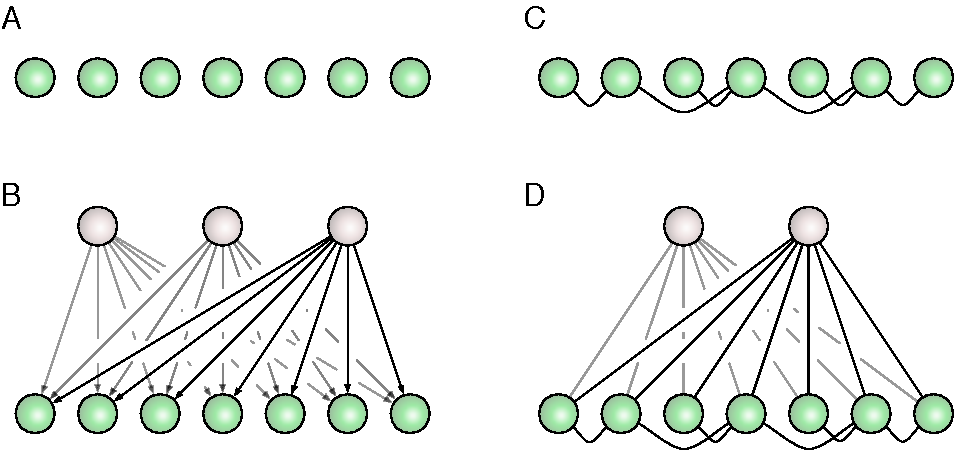
\includegraphics[width=0.6\textwidth]{figures/Figure2.pdf}
\caption{
%\textbf{Figure 2.}{
Graphical models corresponding to the low-dimensional targets of the four regularization schemes used in the paper.
\textbf{A}: A diagonal matrix corresponds to a Gaussian graphical model with no dependencies. 
\textbf{B}: In factor analysis, observed nodes are assumed to be influenced by several latent units (``factors") but are otherwise independent. 
\textbf{C}: In the Gaussian graphical model (also known as the Gaussian Markov Field), correlations arise from sparse pairwise linear interactions between visible units. 
\textbf{D}: In the Gaussian graphical model with latent units, correlations arise  between pairs of nodes 
}\label{fig:02}
%}
\end{figure}

